% Formelsammlung für Datenbanken IT ZHAW IT HS2020

% Dokumenteinstellungen
% ======================================================================

% Dokumentklasse (Schriftgröße 8, DIN A4, Artikel)
\documentclass[8pt,a4paper]{scrartcl}

% Zusätzliche Pakete laden
\usepackage[utf8]{inputenc}		% Zeichenkodierung: UTF-8 (für Umlaute)
\usepackage[german]{babel}		% Deutsche Sprache
\usepackage{multicol}					% Spaltenpaket
\usepackage{amsmath}				% erlaubt mathematische Formeln
\usepackage{amssymb}				% Verschiedene Symbole
\usepackage{graphicx}				% Zum Bilder einfügen benötigt

% Seitenlayout und Ränder:
\usepackage{geometry}
\geometry{a4paper,landscape, left=6mm,right=6mm, top=-1mm, bottom=5mm,includeheadfoot}
\setlength{\parindent}{0mm}

% Dokumentbeschreibung
\title{Formelsammlung Datenbanken ZHAW IT HS2020}
\author{Andreas Sprecher}

% Kopf- und Fußzeile
% ======================================================================
\usepackage{fancyhdr}
\pagestyle{fancy}
\fancyhf{}

\renewcommand{\headrulewidth}{0.0pt}				%obere Linie ausblenden
\renewcommand{\footrulewidth}{0.1pt}					%obere Linie ausblenden

\fancyfoot[L]{Andreas Sprecher}
\fancyfoot[C]{\textbf{Datenbanken}, Seite \thepage}
\fancyfoot[R]{Stand: \todayV}

% Befehle und Befehlsüberschreibungen
% ======================================================================
\renewcommand{\familydefault}{\sfdefault}					% Schriftart SANS für bessere Lesbarkeit bei kleiner Schrift
\renewcommand{\arraystretch}{1.2}								% Array- und Tabellenabstände vergrößern
\newcommand{\todayV}{\the\day.\the\month.\the\year}	%D.M.YYYY

% Dokumentbeginn
% ======================================================================
\begin{document}

	\begin{multicols*}{3}
		\setlength{\columnseprule}{0.4pt}
   		 \parbox{4cm}{
        		\includegraphics[height=2cm]{./img/Logo.jpeg}
  		  }
  		  \parbox{4cm}{
      		  \emph{\Large{Datenbanken}}
   		 }
  		  \vspace{-2mm} 

		\section{Grundlagen}
			\subsection{Daten, Informationen, Wissen}
				\begin{itemize}\itemsep0pt			
					\item Lateinisch datum: gegebenes
					\item Angaben über Dinge und Sachverhalte, die elektronisch gespeichert und verarbeitet werden können
					\item Daten sind strukturierte Zeichen
					\item Daten in einem Kontext sind Informationen
					\item Verknüpfte Informationen zur intellektuellen Einbettung ist Wissen
					\item Dies ist keine präzise Definition
				\end{itemize}
				
			\subsection{Datenmanagement}
				\begin{itemize}\itemsep0pt			
					\item Methodische, konzeptionelle, organisatorische und technische Massnahmen und Verfahren zur Behandlung der Ressource Daten
					\item Daten mit ihrem maximalen Nutzungspotenzial in die Geschäftsprozesse einzubringen
					\item Im laufenden Betrieb die optimale Nutzung der Daten gewährleisten
				\end{itemize}
				
			\subsection{Strukturierte Daten}
				\begin{itemize}\itemsep0pt			
					\item Feste vorgegebene Struktur
					\item Mehrer gleichartige Datensätze mit identischem Aufbau
					\item Gut tabellarisch darstellbar
					\item Relationale Datenbanken
				\end{itemize}
				
					\subsubsection{Unstrukturierte Daten}
						\begin{itemize}\itemsep0pt			
							\item Keine explizite Struktur
							\item Implizite Struktur möglich (Syntax)
							\item Texte, Bilder, Filme, Audiodaten
						\end{itemize}
						
					\subsubsection{Semistrukturierte Daten}
						\begin{itemize}\itemsep0pt			
							\item Teilweise irreguläre bzw. unvollständige Strukturen
							\item Können sich öfters ändern
							\item Schema kann aus zusätzlichen Informationen rekonstruiert werden
							\item Suchergebnise, E-Mail, XML, JSON
						\end{itemize}
						
			\subsection{Persistenz}
				\begin{itemize}\itemsep0pt			
					\item Lateinisch persistere: beharren
					\item Daten über lange Zeit bereitzuhalten
					\item Benötigt nichtflüchtige Speichermedien
					\item Partnerbegriff: Volatilität
				\end{itemize}
				
			\subsection{Datenverwaltung mittels Dateisystemen}
				\begin{itemize}\itemsep0pt			
					\item Speicherung von Daten in Dateien
					\item Anwendungen/Programme lesen/schreiben Daten direkt
					\item Logische und physische Datenabhängigkeit
				\end{itemize}
				
				\subsubsection{Vorteile}
					\begin{itemize}\itemsep0pt		
						\item Einfach, auf Anwendung angepasst, effizient implementierbar
						\item Anwendung muss keine Rücksicht nehmen auf „andere“
						\item Proprietäre (nicht allgemein anerkannten Standards entsprechend) Formate möglich
					\end{itemize}
					
				\subsubsection{Nachteile}
					\begin{itemize}\itemsep0pt		
						\item Probleme bei Mehrfachverwendung der Daten für unterschiedliche Zwecke
						\item Datenstrukturänderung bedeutet i.d.R. Programmänderung
						\item Gleichzeitiger Zugriff aufwändig zu realisieren
						\item Abgestufte Zugriffsrechte aufwändig zu realisieren
						\item Daten werden oft mehrfach gespeichert
						\item Datenaustausch, -integration komplex
					\end{itemize}
					
			\subsection{Datenbanksystem DBS}
				\begin{itemize}\itemsep0pt			
					\item Ein Datenbanksystem DBS ist ein Datenbankverwaltungssystem DBMS inklusive Datenbank
					\item Ein DBS mit Anwendungsprogramm AP ergeben ein Informationssystem IS
				\end{itemize}
				
				\subsubsection{Vorteile}
					\begin{itemize}\itemsep0pt		
						\item Datenkonsistenz (= Datenintegrität) einfacher sicherzustellen
						\item Mehrere Anwendungen können gleichzeitig auf dieselben Daten zugreifen
						\item Anwendungen unabhängig von physischer Datenstruktur
						\item Anwendungen unabhängig von Erweiterungen der Daten
						\item Verwaltung und Nutzung sehr grosser Datenmengen
						\item Deklarativer und mengenorientierter Zugriff
						\item Einmalige, zentrale Datendefinition
						\item Automatisierung wichtiger Aufgaben (Integritätskontrolle, Redundanzverwaltung, Zugriffskontrolle, Zugriffsoptimierung, GleichzeitigerZugriff, Datensicherung und -wiederherstellung)
					\end{itemize}
					
				\subsubsection{Nachteile}
					\begin{itemize}\itemsep0pt		
						\item Aufbau und Betrieb sind anspruchsvoll und teuer
					\end{itemize}
				
			\subsection{Datenbankverwaltungssystem DBMS}
				\begin{itemize}\itemsep0pt				
					\item Effiziente und flexible Verwaltung grosser Mengen persistenter Daten
					\item Werden verwendet um strukturierte Daten zu verwalten
					\item Hoher Grad an Datenunabhängigkeit
					\item Hohe Leistung und Skalierbarkeit
					\item Mächtige Datenmodelle und Abfragesprachen / leichte Handhabbarkeit
					\item Transaktionskonzept (ACID), Datenkontrolle
					\item Ständige Betriebsbereitschaft (hohe Verfügbarkeit und Fehlertoleranz)
				\end{itemize}
				
			\subsection{Relationale Datenbanken}
				\begin{itemize}\itemsep0pt			
					\item Werden verwendet um strukturierte Daten zu verwalten
					\item Bedeutenste Datenbanktechnologie in der Praxis
				\end{itemize}
				
				\subsubsection{Drei Ebenen Architektur}
					\begin{itemize}\itemsep0pt		
						\item Konzeptionell: Logische Gesamtsicht
						\item Extern: Sicht einer Anwendung
						\item Intern: Speicherung, Datenorganisation, Zugriffsstruktur
						\item Realisiert durch ein RDBMS
						\item Datenbeschreibungen ebenfalls in der Datenbank gespeichert
						\item Zwischen den verschiedenen Ebenen (Schemas) erfolgen Transformationen
						\item Logische Datenunabhängigkeit: Externes Schema ändert $\rightarrow$ modifizieren der Transformationsregeln zum konzeptionellen Schema
						\item Physische Datenunabhängigkeit: Internes Schema ändert $\rightarrow$ modifizieren der Transformationsregeln zum konzeptionellen Schema
					\end{itemize}
					
				\subsection{Datenbankentwurf/-betrieb}
					\subsubsection{Aufbau}
						\begin{itemize}\itemsep0pt			
							\item Erstellen von verschiedenen Schemas
							\item Iterativer Prozess
							\item Ausbau und Umbau im laufenden Betrieb typisch
							\item ERM (Entity-Relationship-Model)
							\item DDL (Data Definition Language)
						\end{itemize}
						
					\subsubsection{Betrieb, Benutzung, Verwaltung}
						\begin{itemize}\itemsep0pt			
							\item Abfragen, Einfügen, Ändern und Löschen von Daten
							\item Sicherung und Wiederherstellung
							\item Überwachung und Tuning
							\item Benutzerverwaltung und Rechtevergabe
							\item DML (Data Manipulation Language)
							\item DQL (Data Query Language)
							\item DCL (Data Control Language)
						\end{itemize}
						
						
		\section{Relationenmodell}
			\subsection{Wertebereich (Domäne)}
				\begin{itemize}\itemsep0pt			
					\item Menge einfacher/atomarer Werte
					\item Entspricht im wesentlichen einem Datentyp einer höheren Programmiersprache
					\item Mengen von Werten sind nicht zulässig
				\end{itemize}
					
			\subsection{Attribut}
				\begin{itemize}\itemsep0pt			
					\item Besteht aus Bezeichnung/Name und Domäne/Wertebereich
					\item Ein Attribut nimmt konkrete Werte an
					\item Attributwerte können sich im Laufe der Zeit ändern
					\item Attribute (Name, Bedeutung und Wertebereich) bleiben konstant
				\end{itemize}
					
			\subsection{Tupel (n-Tupel)}
				\begin{itemize}\itemsep0pt			
					\item Sammlung von als zusammengehörig betrachteter Attribute
					\item Feste Zahl von Komponenten
					\item Beliebige Anordnung
					\item Der Attributwert entstammt einer für jedes Attribut festgelegten Domäne
					\item Eine Menge von gleichartig strukturierten Tupeln bildet eine Relation					
				\end{itemize}
				
			\subsection{Relation}
				\begin{itemize}\itemsep0pt			
					\item Besteht aus Relationsschema und Ausprägung
					\item Relationsschema/Format: Menge der Attribute mit Namen und Domäne
					\item Ausprägung: Menge von Tupeln
					\item Eine Relation ist eine Teilmenge des kartesischen Produktes von n endlichen Wertebereichen
					\item Relationen sind Mengen, enthalten also keine doppelten Elemente und sind ungeordnet
					\item Relationen werden oft als Tabellen dargestellt (Domänen werden dabei oft weggelassen)
				\end{itemize}
					
				\subsection{Kurzschreibweisen}
					\begin{itemize}\itemsep0pt			
						\item Kurzschreibweise Format/Schema: R$(A_{1},A_{2},...,A_{n})$
						\item Kurzschreibweise Tupel: $\{<$Max, Muster, Blau$>$,$<$Beni, Beispiel, Rot$>$,$<$Fritz, Müller, Schwarz$>\}$
					\end{itemize}
					
				\subsection{Äquivalenz}
					\begin{itemize}\itemsep0pt			
						\item Enthalten zwei Relationen die gleichen Attribute inklusive Domänen, sind sie äquivalent
						\item R1 $\sim$ R2
					\end{itemize}
					
			\subsection{Schlüssel}
				\subsubsection{Schlüsselkandidat}
					\begin{itemize}\itemsep0pt			
						\item Eine Teilmenge von Attributen K
						\item Es gibt nicht zwei Tupel mit denselben Schlüsselattributwerten in K
						\item In K kann nichts weglassen werden
						\item Wenn mehrere Schlüsselkandidaten zur Verfügung stehen, muss eine Auswahl getroffen werden
					\end{itemize}
					
					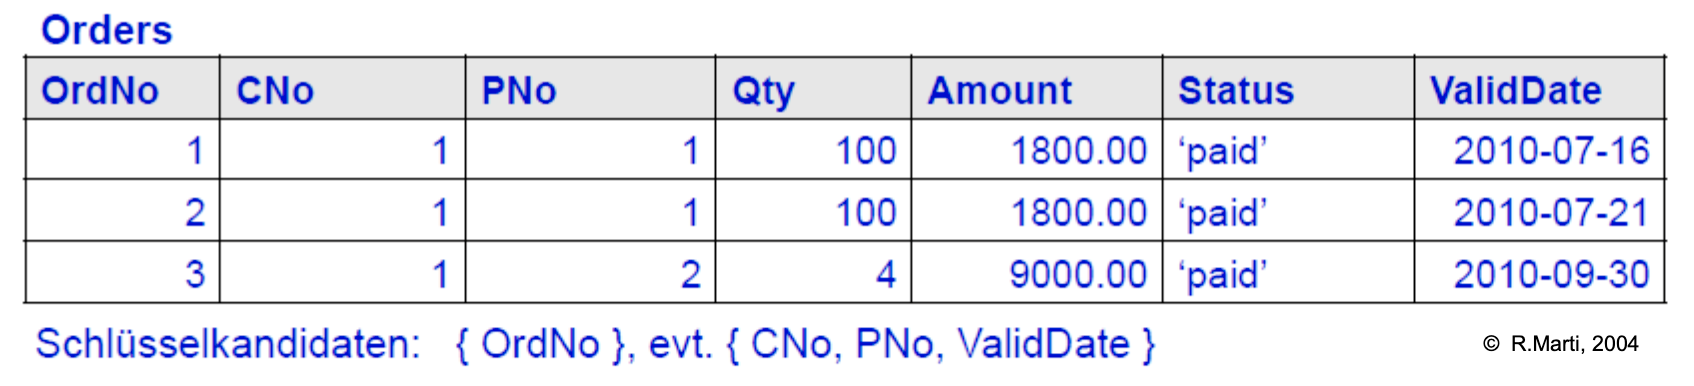
\includegraphics[height=2cm]{img/relationSchluessel.png} 			
					
				\subsubsection{Primärschlüssel}
					\begin{itemize}\itemsep0pt			
						\item Ein ausgewählter Schlüsselkandidat, der explizit als Primärschlüssel bezeichnet wird
						\item Attributwerte sollten sich möglichst wenig ändern
						\item Eindeutigkeit der Werte eines Primärschlüssels sollte über die Zeit gelten
						\item Attribute sollten möglichst wenig Speicherplatz benötigen
						\item Wenn nichts passt Surrogatschlüssel "künstlicher Schlüssel" definieren
					\end{itemize}
					
				\subsubsection{Fremdschlüssel}
					\begin{itemize}\itemsep0pt			
						\item Eine Menge von Attributen in einer Relation S zu der es eine Relation R gibt, deren Primärschlüssel von diesen Attributen in S referenziert werden
						\item Referentielle Integrität: Ein Fremdschlüssel (in S) kann, muss aber nicht Schlüssel in S sein
						\item Primärschlüssel/Fremdschlüssel-Beziehungen müssen explizit deklariert werden
					\end{itemize}		
					
					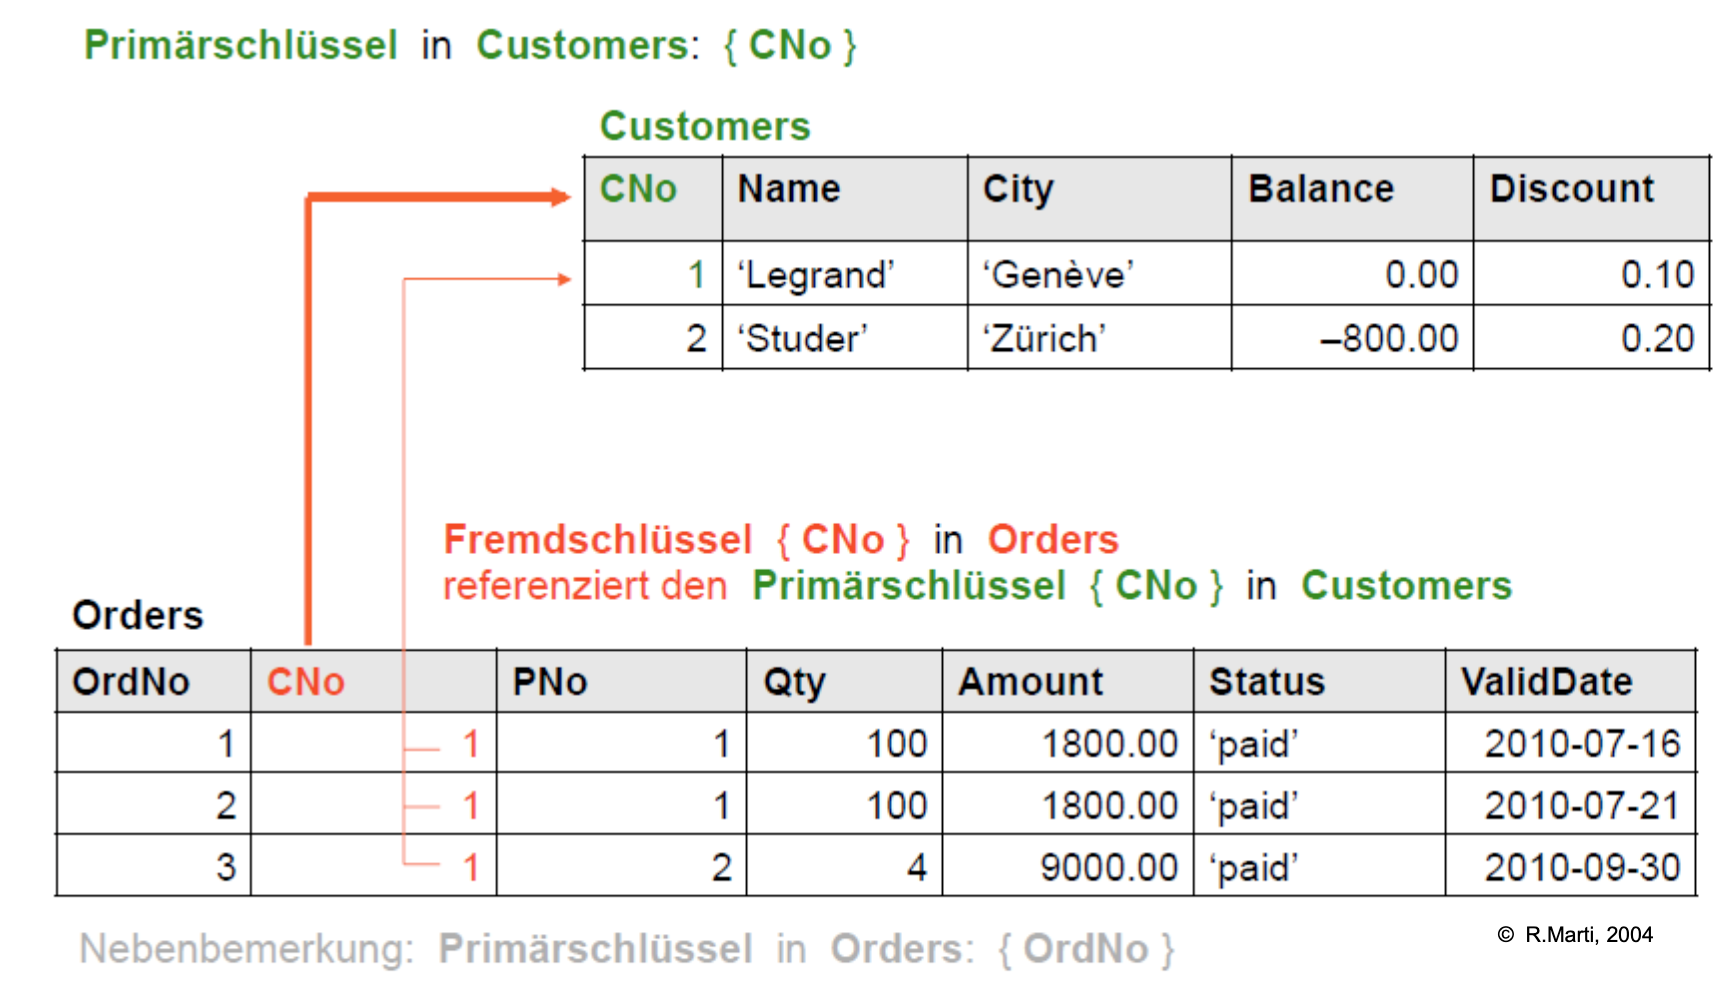
\includegraphics[height=5.25cm]{img/pkfk.png} 	
					
		\section{Relationale Algebra}
			\begin{itemize}\itemsep0pt			
				\item Operatoren und Rechenregeln mit Relationen
				\item Inhalt der Datenbank (Relationen) sind Operanden
				\item Operatoren definieren Funktionen zum Berechnen von Anfrageergebnissen
				\item Rangfolge: $\sigma , \pi , \rho \Rightarrow \times , \bowtie \Rightarrow \cap \Rightarrow\cup , \setminus$
			\end{itemize}
					
			\subsection{Selektion $\sigma$}
				\begin{itemize}\itemsep0pt			
					\item Unärer Operator (d.h. nur ein Operand)
					\item Erzeugt neue Relation mit gleichem Schema aber einer Teilmenge der
Tupel
					\item Nur Tupel, die der sogenannten Selektionsbedingung entsprechen, werden übernommen
					\item Ergebnis kann eine ohne Tupel/leere Relation sein
					\item Selektionsbedingung: Kombination von logischen Ausdrücken bestehend aus Attributen und/oder Konstanten
					\item Prüft Selektionsbedingung für jedes Tupel der Relation
					\item $R' = \sigma_{\text{Selektionsbedingung}}(R)$
					\item $r' = \sigma_{A=0 \vee C=2*B}(r)$
					\item $r' = \sigma_{A=0 \vee C=2*B}(r)$						
				\end{itemize}
				
			\subsection{Projektion $\pi$}
				\begin{itemize}\itemsep0pt			
					\item Unärer Operator (d.h. nur ein Operand)
					\item Erzeugt neue Relation mit einer Teilmenge der ursprünglichen Attribute
					\item Es können Duplikate entstehen, die entfernt werden müssen
					\item Die Projektion wählt eine Menge von Spalten aus
					\item Mit einer Projektion lässt sich auch die Reihenfolge der Spalten anpassen
					\item Die Menge der Attribute muss im Format vorhanden sein, sonst Fehler
					\item $R' = \pi_{\text{A1, A3, A12}}(R)$
					\item $r' = \pi_{\text{Name, Farbe}}(r)$
				\end{itemize}
				
			\subsection{kartesisches Produkt $\times$}
				\begin{itemize}\itemsep0pt			
					\item Kreuzprodukt zweier Relationen R und S
					\item Menge aller Tupel, die entsteht, wenn jeder Tupel aus R mit jedem Tupel aus S kombiniert wird
					\item Schema hat ein Attribut für jedes Attribut aus R und S
					\item Bei Namensgleichheit wird kein Attribut weggelassen,
stattdessen: Umbenennen oder qualifizieren
				\end{itemize}

				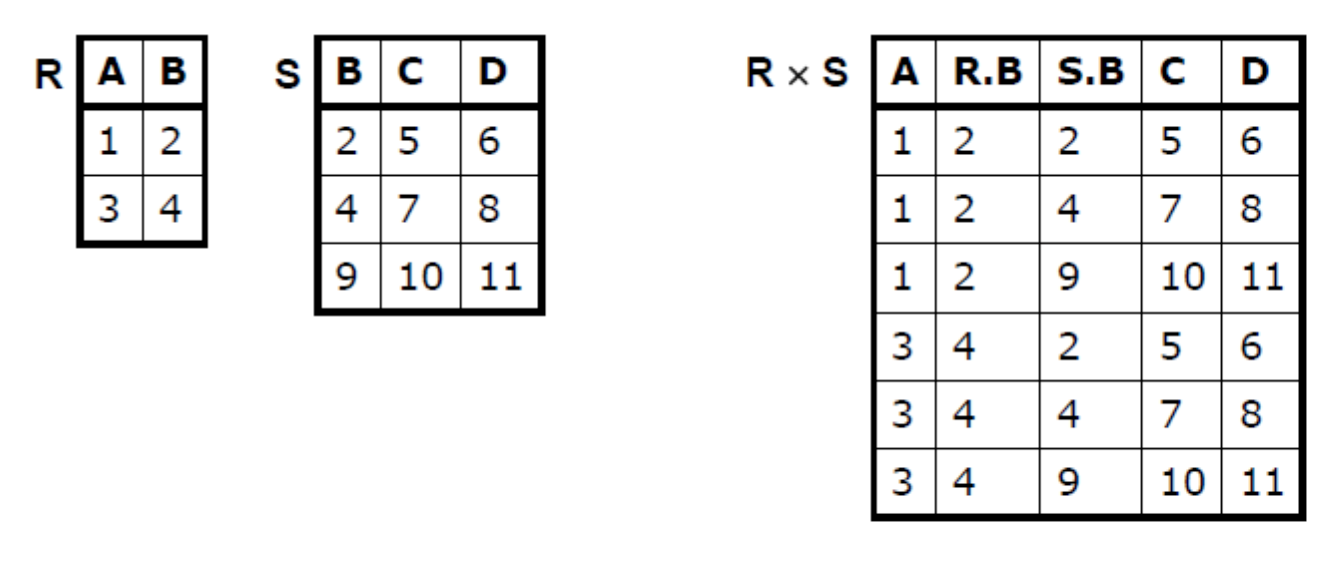
\includegraphics[height=3.5cm]{img/kreuz.png}
				
			\subsection{Verbund, natural Join $\bowtie$}
				\begin{itemize}\itemsep0pt			
					\item Statt im Kreuzprodukt alle Paare zu bilden, sollen nur die Tupelpaare gebildet werden, deren Tupel übereinstimmen
				\end{itemize}

				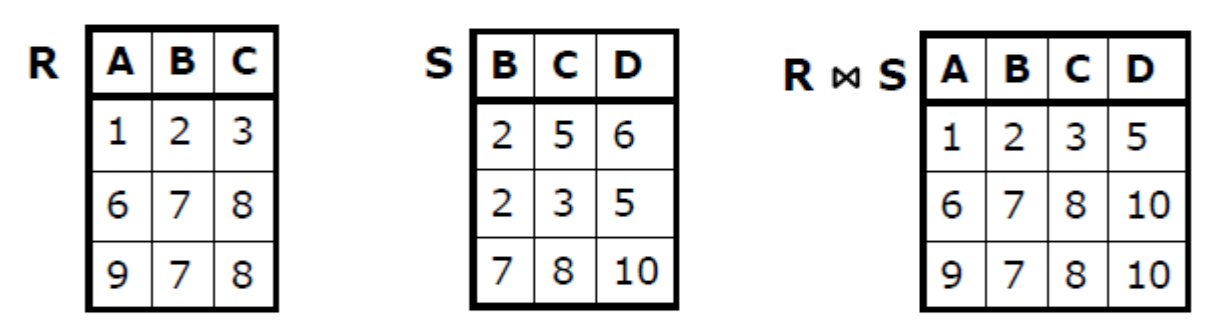
\includegraphics[height=2.5cm]{img/njoin.png}
				
				
			\subsection{Theta Join $\bowtie_{P}$}
				\begin{itemize}\itemsep0pt			
					\item Verallgemeinerung des natürlichen Joins, viel flexibler, darum in der Praxis der Normalfall 
					\item Verknüpfungsbedingung kann frei gestaltet werden
					\item $R \bowtie_{P} S = \sigma_{P}(R \times S)$
				\end{itemize}

				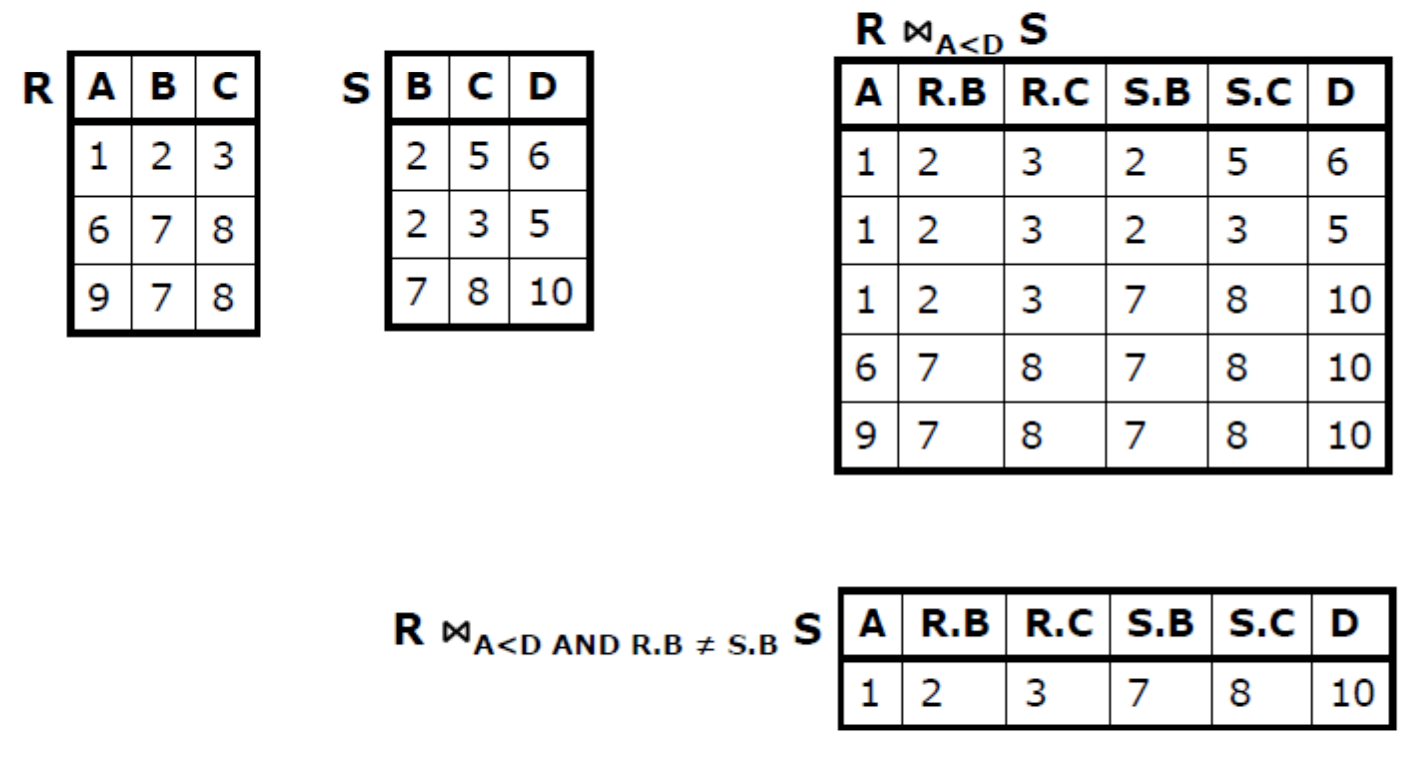
\includegraphics[height=4.5cm]{img/tjoin.png} 	
				
			\subsection{Outer Join}
				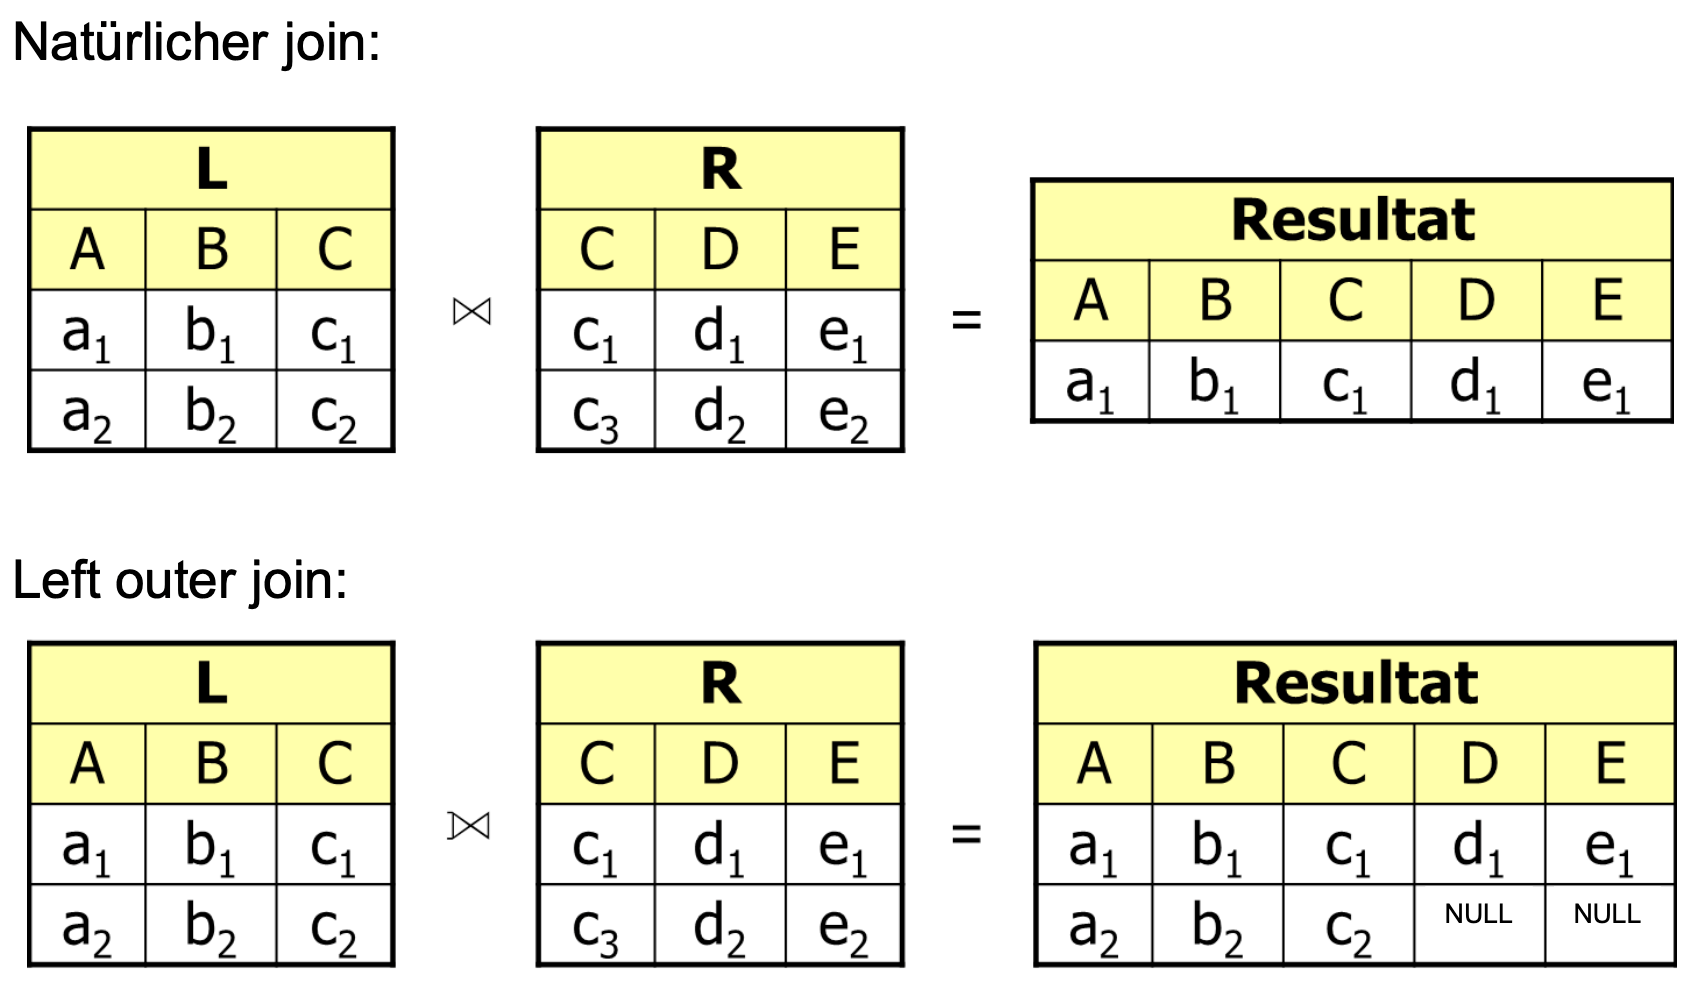
\includegraphics[height=5cm]{img/ojoin1.png}
				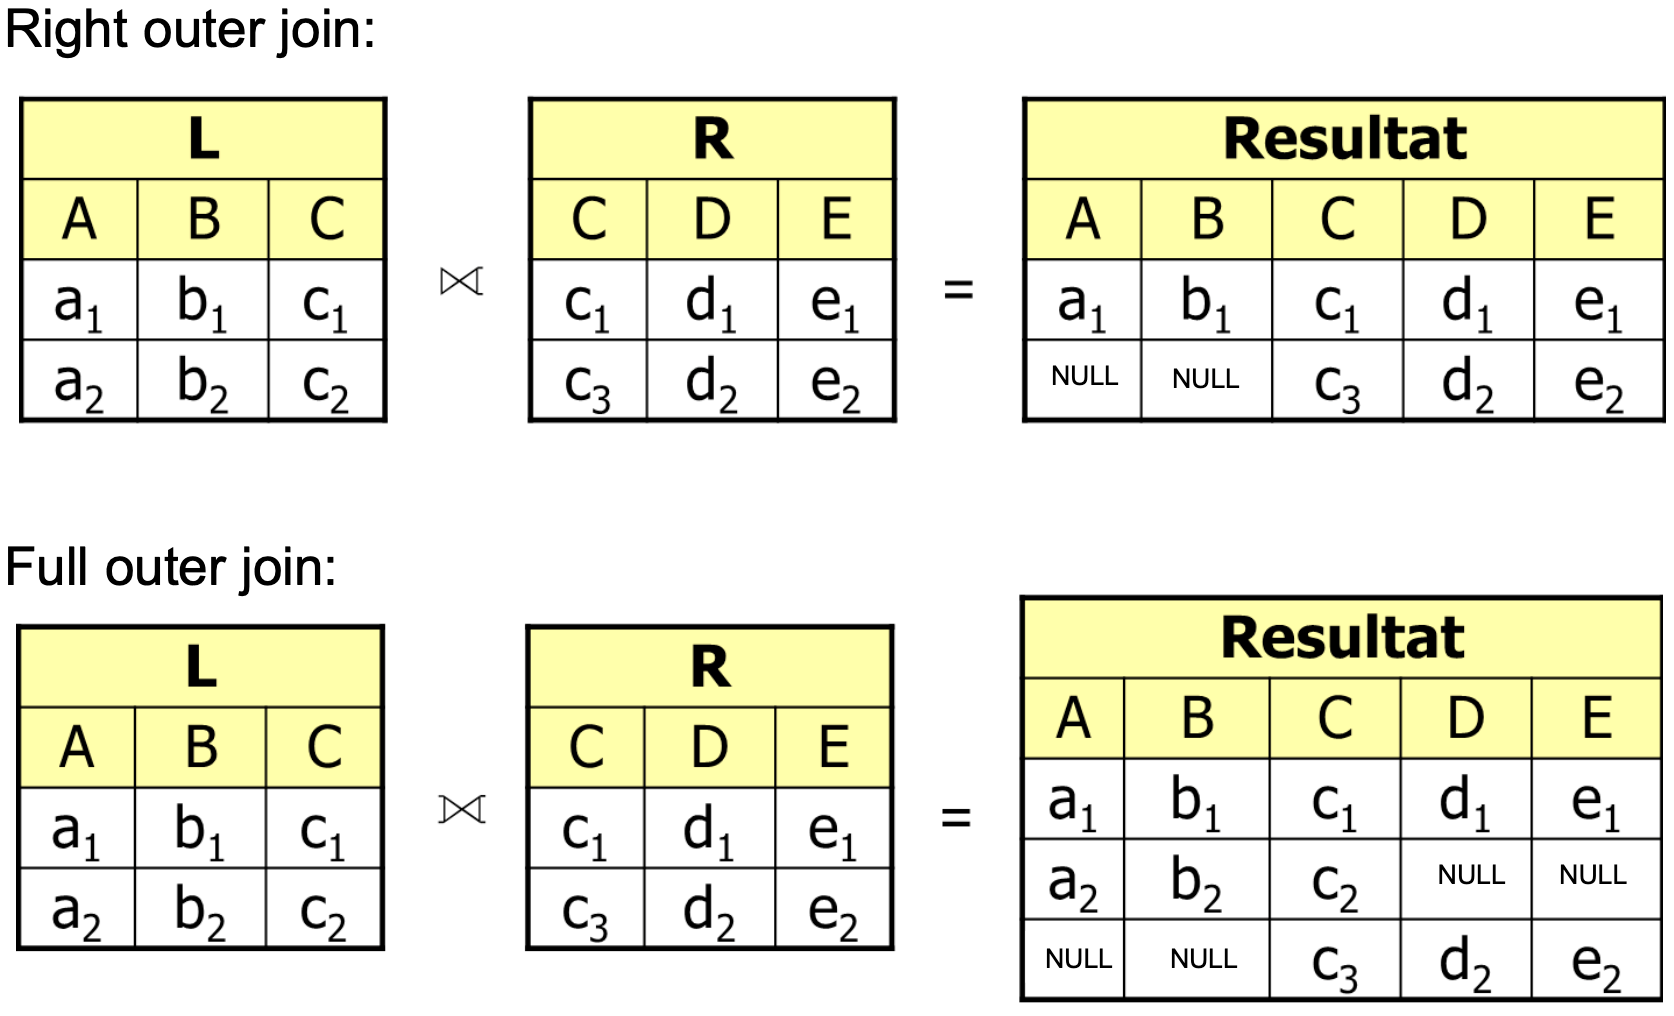
\includegraphics[height=5.25cm]{img/ojoin2.png} 	
		
			\subsection{Mengenoperator}
				\textbf{Vereinigung $\cup$}
				\begin{itemize}\itemsep0pt			
					\item  $R \cup S$
					\item Müssen gleiches Schema haben
					\item Tupel die in R oder S vorkommen ohne Duplikate
				\end{itemize}
				
				\textbf{Differenz $\setminus$}
				\begin{itemize}\itemsep0pt		
					\item R $\setminus$ S oder R - S
					\item Müssen gleiches Schema haben
					\item Tupel die in R aber nicht in S vorkommen
				\end{itemize}
				
				\textbf{Durchschnitt $\cap$}
				\begin{itemize}\itemsep0pt		
					\item R $\cap$ S
					\item Müssen gleiches Schema haben
					\item Tupel die in R und S vorkommen
				\end{itemize}
				
			\subsection{Qualifizierung, Namenskonflikte $\rho$}
				\begin{itemize}\itemsep0pt			
					\item  $\rho_{S(D,E)}(R(A,B))$
					\item Aus R(A,B) wird S(D,E)
				\end{itemize}
			
				
			\subsection{Äquivalenzen}
				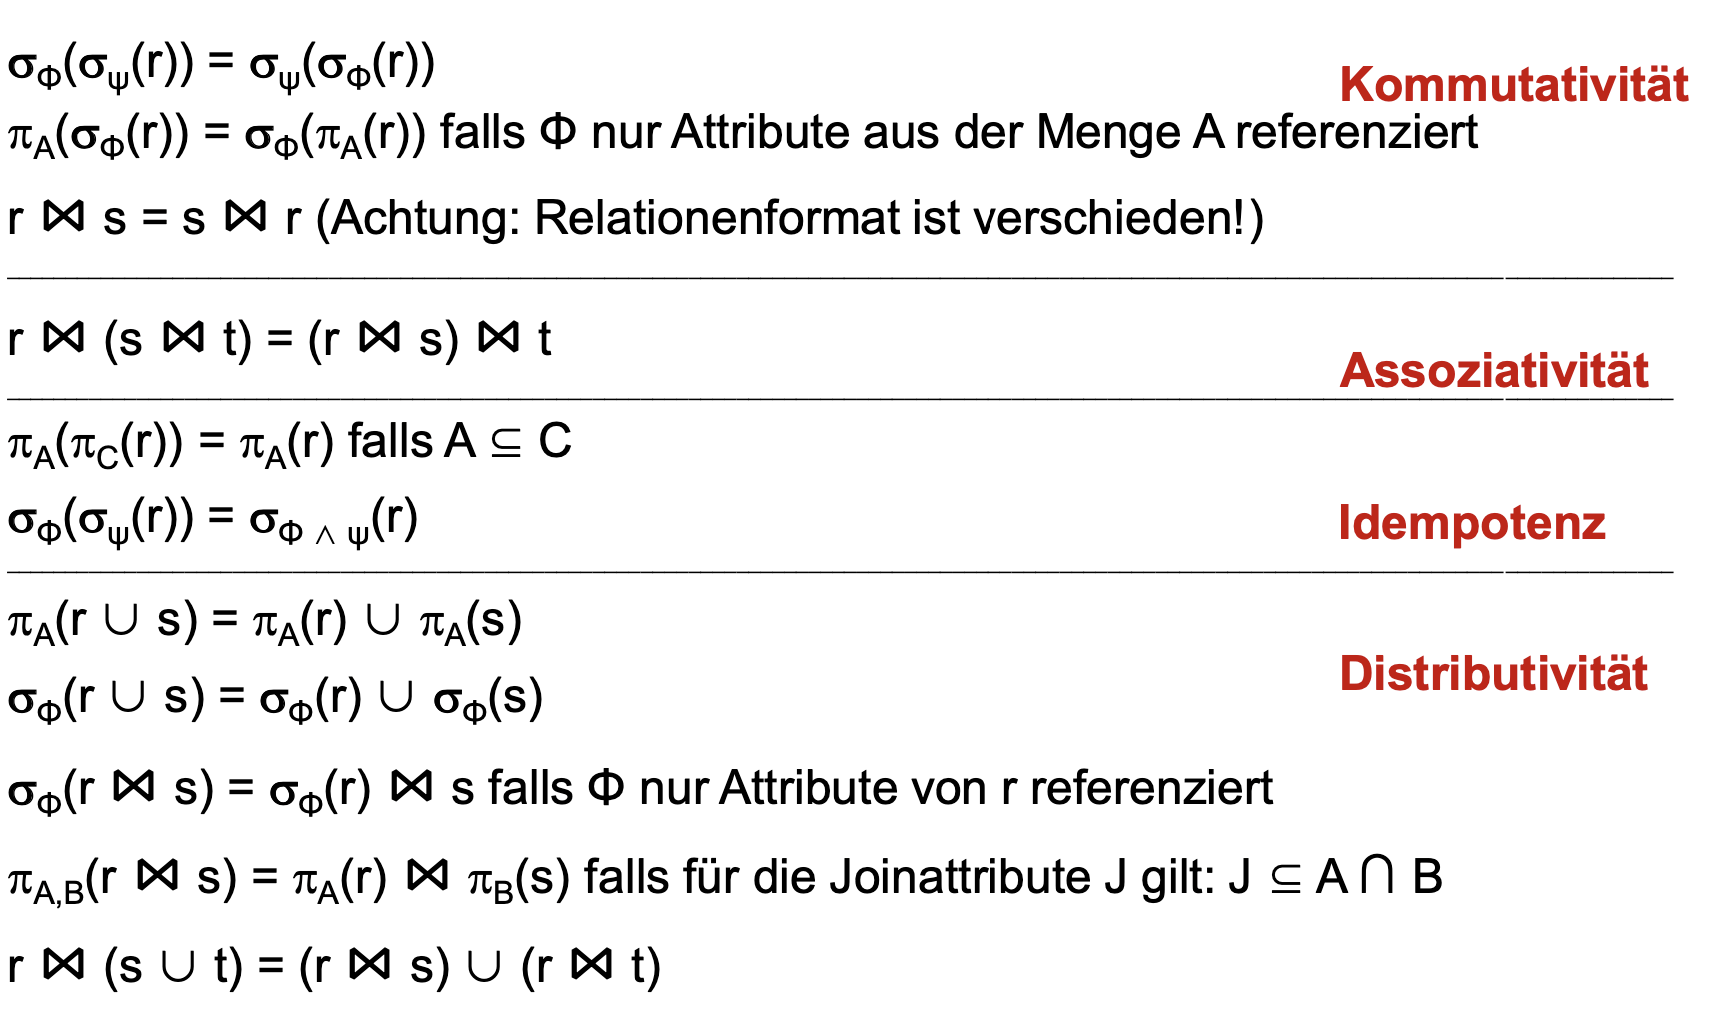
\includegraphics[height=5.5cm]{img/aequivalenzen.png}
				
				
			\subsection{Aggregat-Funktionen}
				\subsubsection{Summe $\Sigma$}
					\begin{itemize}\itemsep0pt			
						\item R(A,B,X) und S(A)
						\item $r = \{<a1,b1,2>,<a1,b2,3>,<a2,b1,4>\}$
						\item $\Sigma_{X}(r)=\{<9>\} $
						\item Gruppieren: $\Sigma_{S,X}(r)=\{<a1,5>,<a2,4>\} $
					\end{itemize}
					
				\subsubsection{Aggregats-Operator F}
					\begin{itemize}\itemsep0pt			
						\item $F_{\text{COUNT}}$: Anzahl Tupel
						\item $F_{\text{MAX}}$: Grösster Wert des betrachteten Attributs
						\item $F_{\text{MIN}}$: Kleinster Wert des betrachteten Attributs
						\item $F_{\text{SUM}}$: Summe des betrachteten Attributs
						\item $F_{\text{AVG}}$: Durchschnitt des betrachteten Attributs
					\end{itemize}

		\section{Entity-Relationship Design}
			\subsection{3-Phasen}
				\begin{itemize}\itemsep0pt			
					\item Konzeptionelle Datenmodell: weitgehend technologieunabhängige Spezifikation der Daten
					\item Logische Datenmodell: Übersetzung des konzeptionellen Schemas in Strukturen, die mit einem konkreten DBMS implementiert werden können
					\item Physische Datenmodell: Anpassungen, die nötig sind um eine befriedigende Leistung im Betrieb zu erreichen (Datenverteilung, Performanz, Sicherheit, ...)
				\end{itemize}
				
			\subsection{Konzeptioneller Entwurf}
				\begin{itemize}\itemsep0pt			
					\item Klassifikation: Identifikation von gleichen oder ähnlichen Eigenschaften
					\item Aggregation: Zusammenfassen von diesen Eigenschaften
					\item Generalisierung und Spezialisierung: Verallgemeinerung (Student $\rightarrow$ Person)
				\end{itemize}
						
			\subsection{Entität}
				\begin{itemize}\itemsep0pt			
					\item Konkretes oder abstraktes Objekt, welches eindeutig identifiziert werden kann
					\item Ein \textbf{Entitätstyp} steht für Mengen von gleichartigen Entitäten
					\item Darstellung durch Rechteck mit eindeutigem Namen
					\item Ein Entitätstyp wird später in eine Tabelle mit Schlüsseln abgebildet, die Entitäten werden die Zeilen der Tabelle sein
					\item Entitätstypen haben Eigenschaften (Attribute)
					\item Entitäten haben Attributwerte
					\item Attribute werden als Ovale dargestellt
					\item Unterstrichene Attribute sind Primärschlüssel 
					\item Jeder unabhängige Entitätstyp erhält einen oder mehrere Schlüssel
					\item Falls der Entitätstyp eingehende Pfeile hat, wird ein Primärschlüssel bestimmt
				\end{itemize}
				
			\subsection{Beziehungstyp}
				\begin{itemize}\itemsep0pt			
					\item Wird durch einen Rhombus dargestellt
					\item Erbt die Primärschlüsselattribute der Entitätstypen von denen er abhängig ist
					\item m bedeutet beliebig viele, auch 0
				\end{itemize}
				
				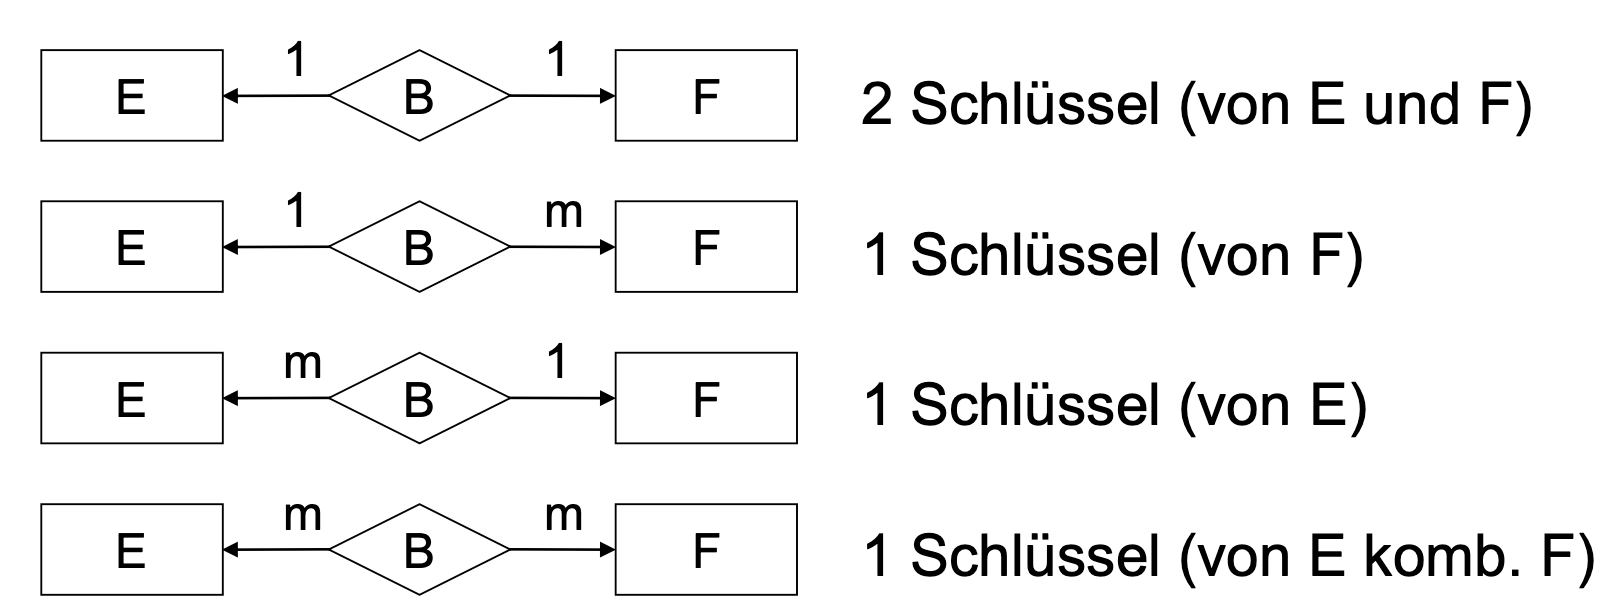
\includegraphics[height=3.5cm]{img/beziehungkey.png}\\
				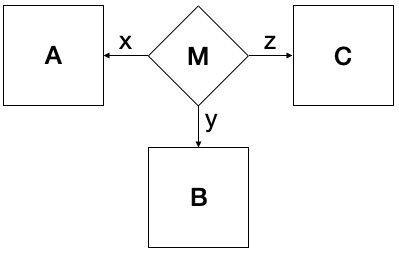
\includegraphics[height=5.9cm]{img/3kardi1.png}\\
				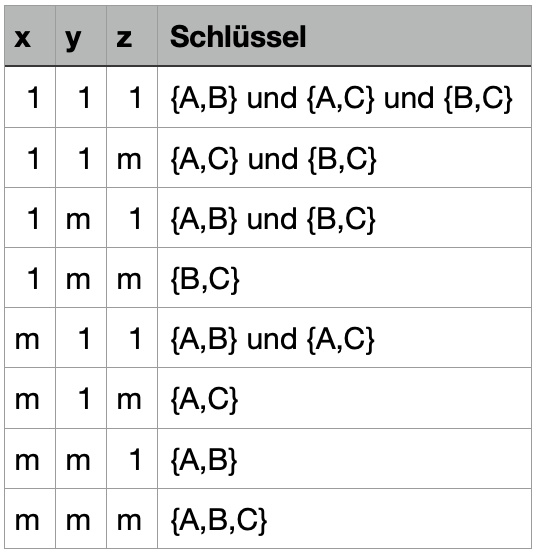
\includegraphics[height=9.5cm]{img/3kardi2.png}
		
	
			\subsection{ISA-abhängiger Entitätstyp}
				\begin{itemize}\itemsep0pt			
					\item Ein ISA-abhängiger Entitätstyp ist eine Untergruppe eines anderen Entitätstyps
					\item 1:1 Relation
				\end{itemize}
				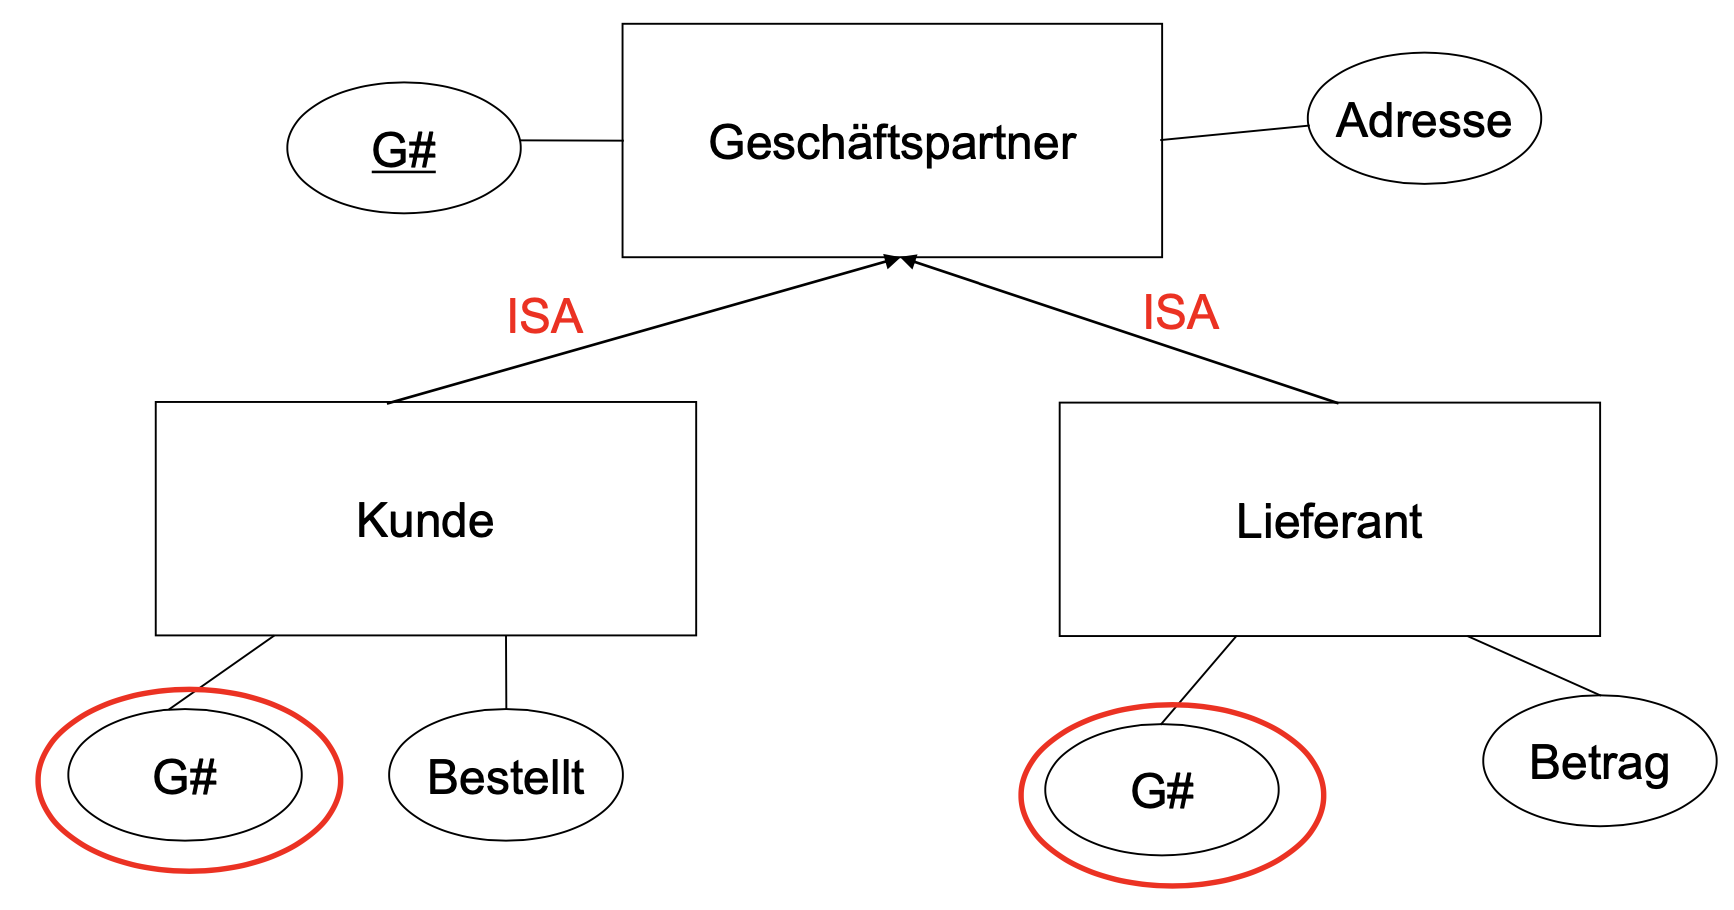
\includegraphics[height=4.8cm]{img/ISA.png}
				
			\subsection{ID-abhängiger Entitätstyp}
				\begin{itemize}\itemsep0pt			
					\item Ein ID-abhängiger Entitätstyp ist eine Untergruppe eines anderen Entitätstyps
					\item Komplexe Attribute führen zu ID-abhängigen Entitätstypen
					\item 1:M Relation
				\end{itemize}
				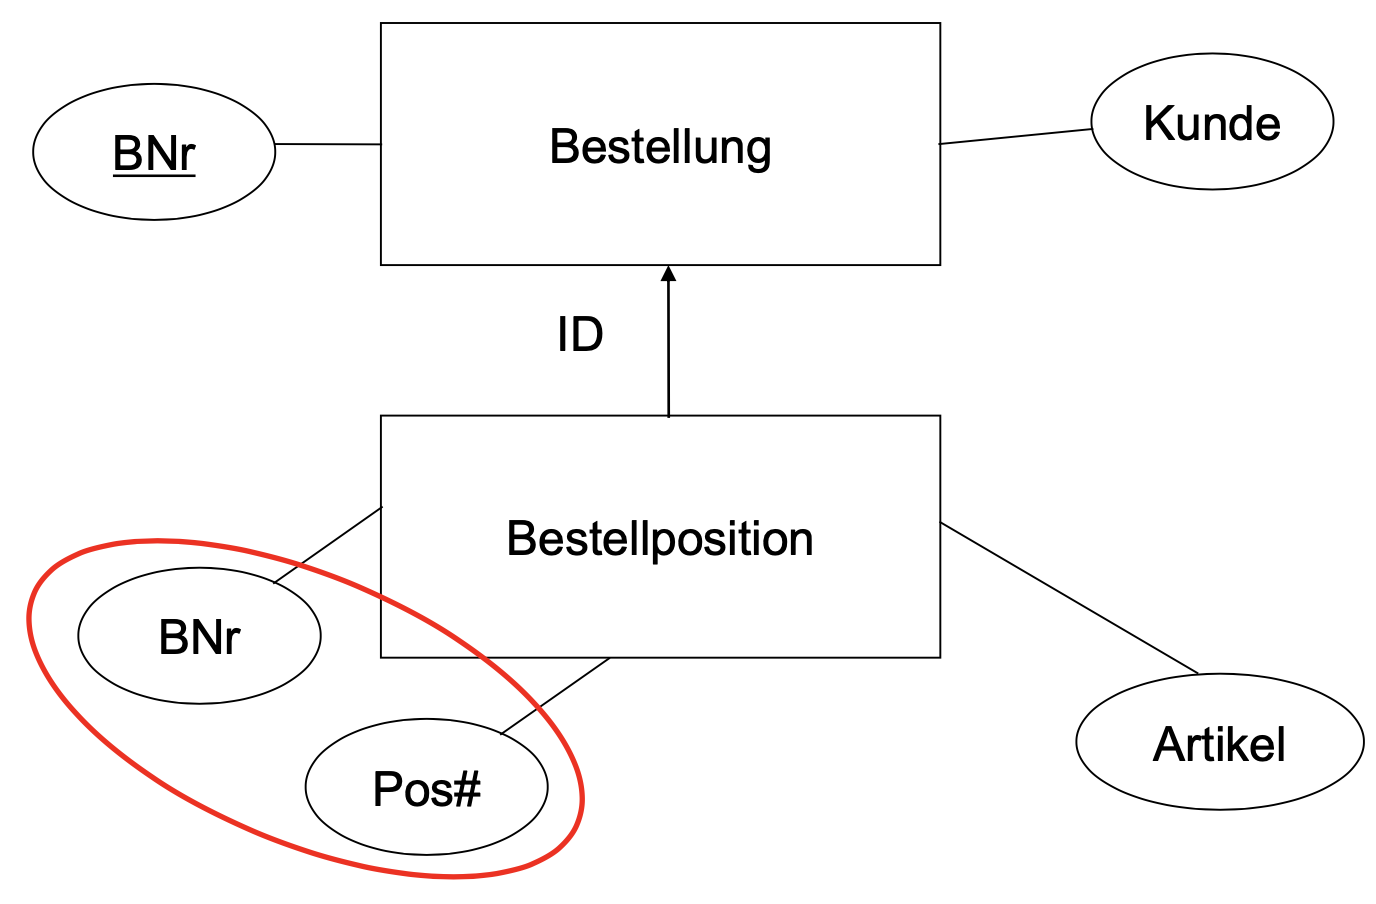
\includegraphics[height=6cm]{img/ID.png}
				
			\subsection{Zusammengesetzter Entitätstyp}
				\begin{itemize}\itemsep0pt		
					\item Wird verwendet, wenn an Beziehungstypen Entitätstypen angehängt werden wollen	
					\item Es wird ein Rechteck um den Beziehungstyp gezeichnet
				\end{itemize}
		
		
			\subsection{Anomalien}
				\subsubsection{Update-Anomalien}
					\begin{itemize}\itemsep0pt		
						\item Sachverhalt in der Realität ändert sich
						\item Mehrere Änderungen in einer Relation sind nötig
					\end{itemize}
				\subsubsection{Delete-Anomalien}
					\begin{itemize}\itemsep0pt		
						\item Sachverhalt in der Realität ändert sich
						\item Information in einer Relation verschwindet
					\end{itemize}
				\subsubsection{Insert-Anomalien}
					\begin{itemize}\itemsep0pt		
						\item Sachverhalt der Realität möchte abgebildet werden
						\item Information kann nicht erfasst werden
					\end{itemize}
				\subsubsection{Normalisieren}
					\begin{itemize}\itemsep0pt		
						\item Bei der Normalisierung werden Relationen aufgeteilt
						\item Ist ein mathematischer Prozess
					\end{itemize}
		
		\section{SQL}
			\subsection{Mängel}
				\begin{itemize}\itemsep0pt		
					\item Mangelnde Performanz (in den siebziger Jahren) führte zu Kompromissen
					\item Verzicht auf eine rein mengenmässige Verarbeitung
					\item SQL lässt Duplikate zu
					\item Die Behandlung von NULL
					\item Trotz Standardisierungsbemühungen ist eine Vielzahl von Dialekten entstanden
					\item Die Sprache enthält sehr viel Redundanz
				\end{itemize}
				
			\subsection{ER-Schema zu Relationenformat}
				\begin{itemize}\itemsep0pt		
					\item Jeder Entitäts- und jeder Beziehungstyp ergibt ein Relationenformat, unabhängige Entitätstypen zuerst
					\item Alle Fremdschlüssel-Attribute müssen im Relationenformat aufgeführt werden
					\item Primärschlüssel-Attribute werden auch bei der Dokumentation des Relationenformats unterstrichen
					\item Es ist empfehlenswert jeder Tabelle einen Primärschlüssel zuzuweisen
				\end{itemize}
				
			\subsection{Relationenformat zu Tabellen}
				\begin{itemize}\itemsep0pt		
					\item Jedes Relationenformat wird zu einer Datenbank-Tabelle
					\item Die Tupel in einer Tabelle sind \textbf{nicht} geordnet
					\item <A, B> und <B, A> sind verschiedene Schlüssel
					\item Unique-Schlüssel ist nötig 
					\item Es ist empfehlenswert, immer einen Primärschlüssel zu definieren
					 
				\end{itemize}
				
			\subsection{Data Definition Language DDL}
				\begin{itemize}\itemsep0pt		
					\item Erzeugen, Ändern, Löschen von Datenbankobjekten
					\item CREATE, ALTER, DROP,...
				\end{itemize}
				
				\subsubsection{CREATE TABLE}
					\begin{itemize}\itemsep0pt		
						\item Es kann höchstens einen PK pro Tabelle geben
						\item Es sind mehrere Unique-Klauseln pro Tabelle möglich
						\item Es ist abzuraten, andere Attribute als den PK als FK zu referenzieren
						\item Anhand der Referenz sichert das DBMS bei Dateneingabe, aber auch bei Löschen von Tabellen, die referentielle Integrität
						\item Trigger: ON DELETE, ON UPDATE wenn ein Tupel in der referenzierten Tabelle gelöscht, geändert oder eingefügt wird
						\item Trigger: CASCADE Werte des Fremdschlüssels werden bei Ändern des PK-Werts der referenzierten Tabelle automatisch angepasst
						
					\end{itemize}		
					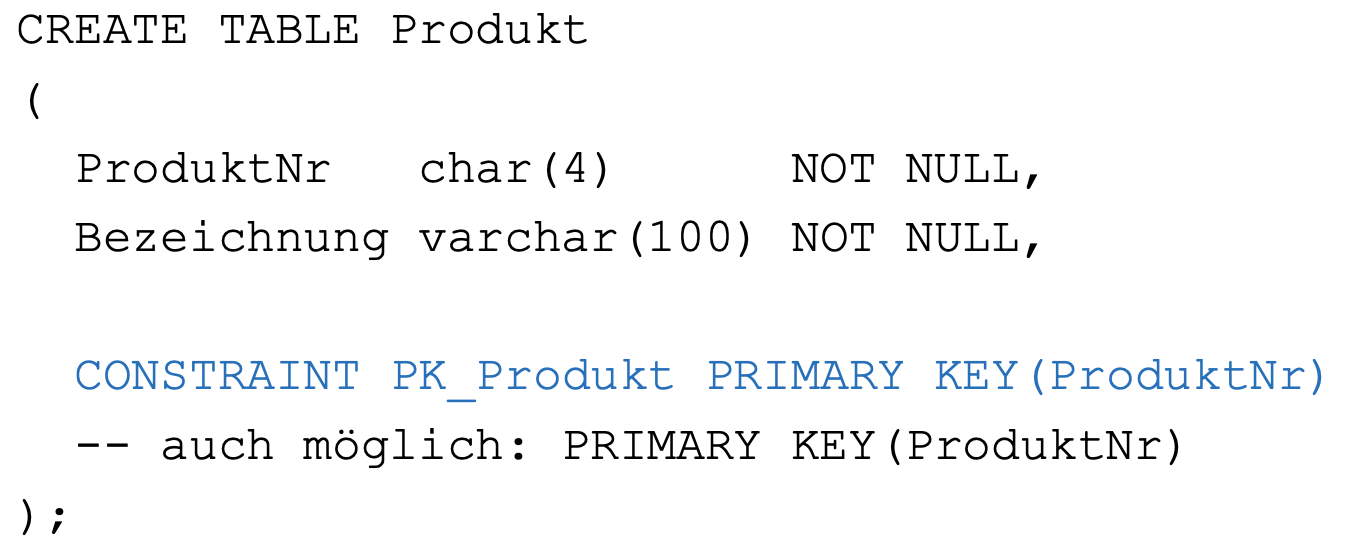
\includegraphics[height=3.5cm]{img/createTablePk.png}
					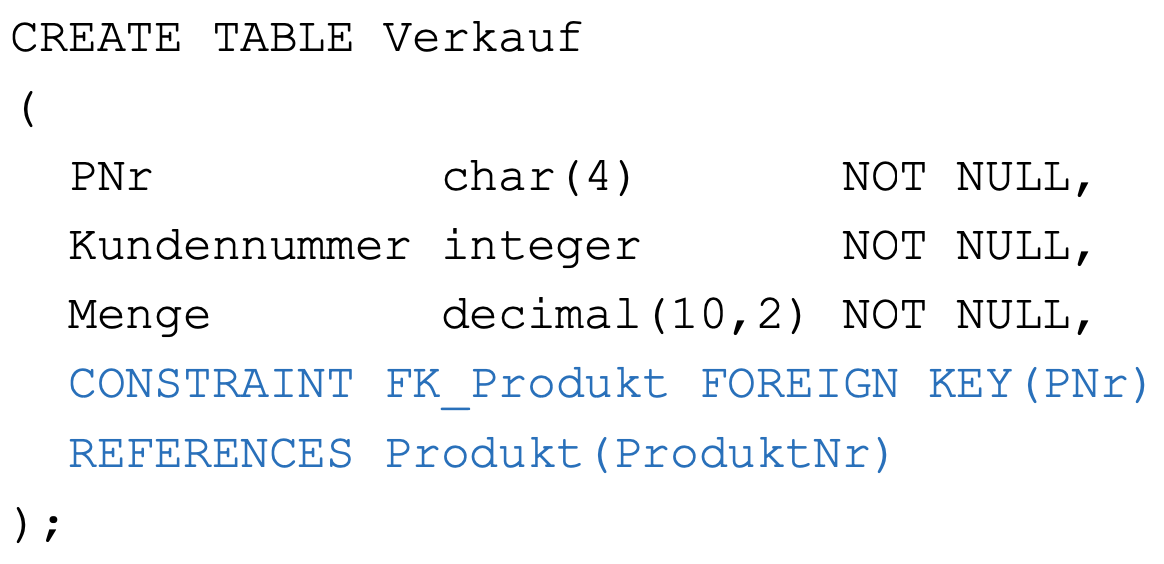
\includegraphics[height=3.8cm]{img/createTableFk.png}
				
				\subsubsection{ALTER TABLE}
					\begin{itemize}\itemsep0pt		
						\item Wenn eine Datenbank sauber implementiert und richtig genutz wird, kann sie im laufenden Betrieb erweitert werden
						\item ALTER TABLE Verkauf ADD Datum date NOT NULL$;$
						\item ALTER TABLE Verkauf ADD CONSTRAINT FK\_Kunde FOREIGN KEY (KundenNummer) REFERENCES Kunde(KNr)$;$
					\end{itemize}		
					
				\subsubsection{DROP TABLE}
					\begin{itemize}\itemsep0pt		
						\item Löschen von Tabellen
						\item DROP TABLE Verkauf$;$
					\end{itemize}	

			\subsection{Data Manipulation Language DML}
				\begin{itemize}\itemsep0pt		
					\item Datenändern (Einfügen,Ändern,Löschen)
					\item INSERT, UPDATE, DELETE, ...
				\end{itemize}	
				
				\subsubsection{INSERT}
					\begin{itemize}\itemsep0pt		
						\item Anzahl und Datentypen müssen zueinander passen
						\item Die Attributnamen können weggelassen werden, ist aber schlechter Stil
						\item Bei fehlenden Attributwerten wird der Default-Wert (oder NULL) eingetragen
						\item Bei unzulässigen Daten wird nichts eingefügt
						\item INSERT INTO Student (SNo,SName,Adresse) VALUES ('87-604-1','Meier','Basel')$;$
						\item Es kann auch das Resultat einer Abfrage eingefügt werden
						\item INSERT INTO Employees (EmpFirstName, EmpLastName) SELECT Customers.CustFirstName,
Customers.CustLastName FROM Customers WHERE Customers.CustomerID IN (1,4,9)$;$
					\end{itemize}	
					
				\subsubsection{UPDATE}
					\begin{itemize}\itemsep0pt		
						\item UPDATE wird in der Regel mit einer Selektion verbunden
						\item UPDATE Student SET Adresse = 'Zürich' WHERE SNo = '87-604-1'$;$
						\item Es können mehrere Attributwerte in einer Anweisung gleichzeitig geändert werden
						\item Wenn die WHERE-Klausel weggelassen wird, werden ALLE Tupel geändert
						\item Bei unzulässigen Daten wird nichts geändert
						\item Für die neuen Attributwerte können auch Berechnungen (*, /, -, +) mit bereits
bestehenden Attributwerten gemacht werden
						\item UPDATE Belegt SET Note = Note + 0.5 WHERE SNo = '87-604-1'$;$
					\end{itemize}	
					
				\subsubsection{DELETE}
					\begin{itemize}\itemsep0pt		
						\item DELETE löscht immer ganze Tupel
						\item DELETE wird in der Regel mit einer Selektion verbunden
						\item Ohne Search Condition/WHERE-Klausel wird die ganze Tabelle geleert
						\item DELETE FROM Salaer WHERE Betrag > 100000;
						\item Bei Verletzung von Schlüsselbedingungen oder wenn die WHERE-Klausel
keine Treffer ergibt, wird nichts gelöscht
					\end{itemize}	
				
			\subsection{Data Query Language DQL}
				\begin{itemize}\itemsep0pt		
					\item Daten lesen (Anfragen an Datenbank stellen)
					\item SELECT – FROM – WHERE
					\item Bei Duplikaten erhält man einen relationalen Bag
				\end{itemize}			
				
				\subsubsection{SELECT}
					\begin{itemize}\itemsep0pt		
						\item Entspricht der Projektion
					\end{itemize}	
			
			\subsection{Data Control Language DCL}
				\begin{itemize}\itemsep0pt		
					\item Rechtevergabe, Datensicherung, ...
					\item GRANT, REVOKE, ...
				\end{itemize}		
				
			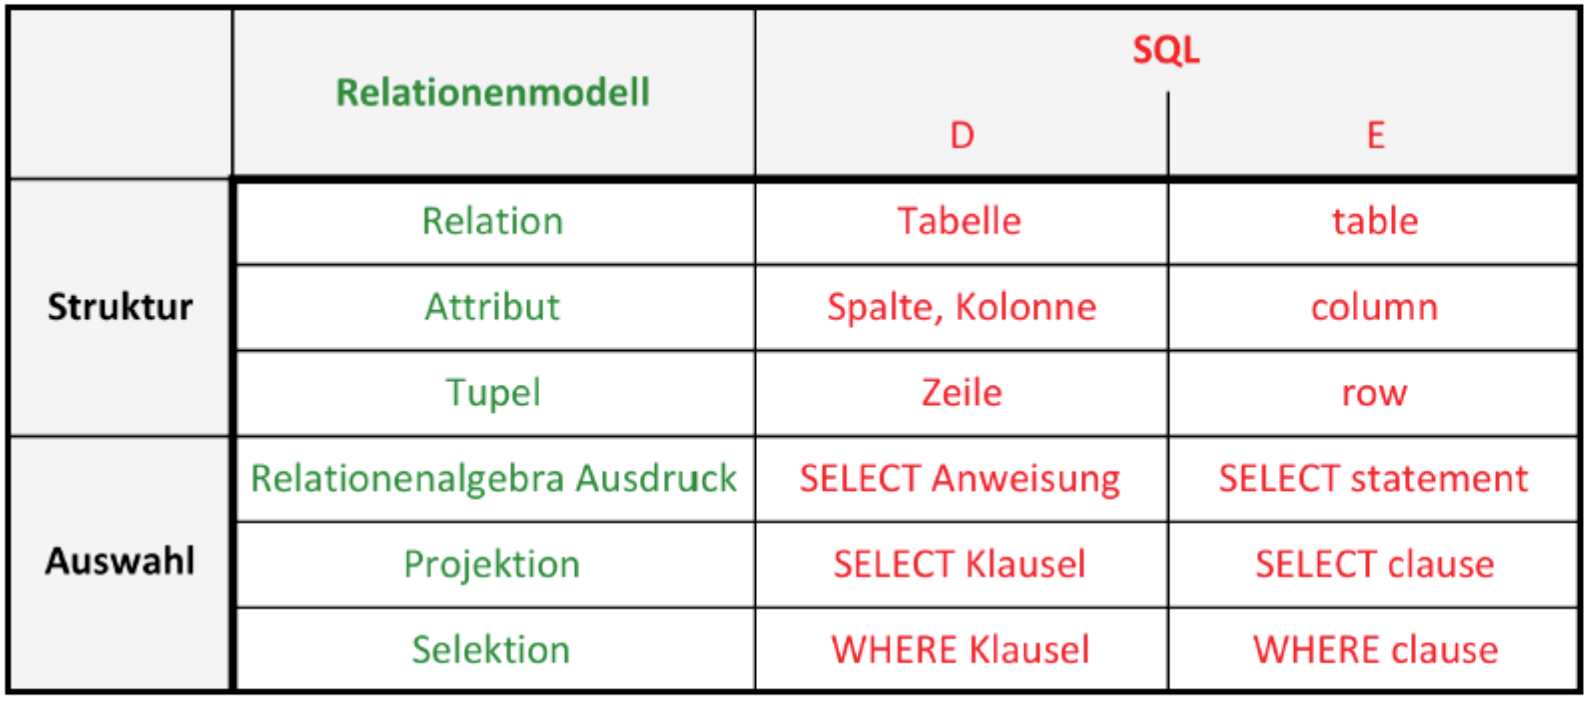
\includegraphics[height=4cm]{img/sql1.png}
			
			\subsection{Syntaxregeln}
				\begin{itemize}\itemsep0pt		
					\item SQL ist keine Mengensprache, sondern eine Sprache für den Umgang mit relationalen Bags
					\item In SQL spielt Gross-/Kleinschreibung nur innerhalb von Text-Konstanten eine Rolle
					\item Konvention: Schlüsselworte gross schreiben (z.B. CREATE TABLE)
					\item Konvention: Schemaelemente klein schreiben (ausser am Wortanfang)
					\item Ein Name (TableName, TableAlias, ColumnName, ColumnAlias, ...) muss mit einem Buchstaben beginnen, gefolgt von Buchstaben, Ziffern oder der Unterlänge (underscore) \_
					\item Jede Anweisung ist mit einem $;$ (Semikolon) abzuschliessen.
				\end{itemize}	
			
			
			
				
				
				
				
				
				
				
				
		
		\section{Technische Aspekte}
		
	\end{multicols*}
\end{document}